\documentclass[11pt,a4paper]{article}

\usepackage[utf8]{inputenc}
\usepackage[T1]{fontenc}
\usepackage[english]{babel}
\usepackage{amsmath,amssymb}
\usepackage[top=1.2cm,bottom=1.5cm,left=2cm,right=2cm]{geometry}
\usepackage{graphicx}
\usepackage{booktabs}
\usepackage{hyperref}
\hypersetup{colorlinks=true,linkcolor=black,citecolor=blue,urlcolor=blue}

\title{Question A --- The Competing Race Between Repair and Detection}
\author{Alexandre Boyer}
\date{}

\begin{document}
\maketitle

\noindent We formalize and bound $P(\tau_{\mathrm{ARF}} < \tau_{\mathrm{det}})$ without
any assumption on the dependence between the two clocks. Notation reminder: $\tau^*$
is the (known) drift instant ; $\tau_{\mathrm{ARF}}$ the delay until the first tree is
replaced, $\min_i \tau_i$ over $M$ trees ; $\tau_{\mathrm{det}}$ the delay until the
first external alarm, possibly $+\infty$ ; $F_A$ and $F_D$ the cumulative distribution
functions of $\tau_{\mathrm{ARF}}$ and $\tau_{\mathrm{det}}$ respectively ; $H$ the
post-drift observation horizon ($H = 2{,}000$) ; $\mathrm{Miss}$ the ``blind spot''
event, defined in Section~1.

\section{Probability Space and Boundary Cases}

\paragraph{The double-starvation case.} The event
$\{\tau_{\mathrm{ARF}}=+\infty,\ \tau_{\mathrm{det}}=+\infty\}$ describes a run where
neither did the forest ever repair itself, nor did the alarm ever sound. This is
qualitatively different from the paradox under study: the blind spot narrative relies
on a \emph{silent} repair erasing the evidence before the alarm gets its chance. If the
repair itself never happened, there is nothing to erase --- the model simply remains
broken, with no mechanism having ``cheated''. With the natural definition
$\mathrm{Miss} := \{\tau_{\mathrm{ARF}} < \tau_{\mathrm{det}}\}$ on the extended reals,
the strict inequality $\infty < \infty$ is false by convention: double starvation is
therefore automatically excluded from $\mathrm{Miss}$, with no special handling needed.

\paragraph{Strict or non-strict inequality?} The stream is discrete: two processes can
legitimately land on the same time step, so $P(\tau_{\mathrm{ARF}}=\tau_{\mathrm{det}})$
can be strictly positive --- the question is not cosmetic. Physical interpretation of an
equality $\tau_{\mathrm{ARF}}=\tau_{\mathrm{det}}=t$: the alarm sounds \emph{exactly}
when the forest repairs itself, the operator is informed at the same instant, no
information is lost --- unlike the true blind spot, where the alarm arrives too late or
never. An equality should therefore count as a detection success.

\begin{center}
\fbox{\parbox{0.93\textwidth}{\textbf{Adopted convention.}
\[ \mathrm{Miss} := \{\tau_{\mathrm{ARF}} < \tau_{\mathrm{det}}\} \qquad \text{(strict inequality)} \]
A tie is classified on the detector's side. Both clocks count integer steps, so
ties are not ruled out by any continuity argument: their frequency has to be measured,
and it is, in Section~4.}}
\end{center}

\section{Identification Under a Finite Horizon}

Absolute censoring is the event
$C_H := \{\min(\tau_{\mathrm{ARF}},\tau_{\mathrm{det}}) > H\}$: neither event has
happened yet at the horizon, so the winner of the race is unobservable. Conversely
$\{\tau_{\mathrm{ARF}}\le H\}$ and $\{\tau_{\mathrm{det}}\le H\}$ are observable.

\paragraph{Four-region partition.} Every run falls into exactly one of the following
four cases.

\begin{center}
\begin{tabular}{cccl}
\toprule
Region & $\tau_{\mathrm{ARF}}$ observed? & $\tau_{\mathrm{det}}$ observed? & Verdict \\
\midrule
1 & $\le H$ & $\le H$ & Miss decided directly (direct comparison) \\
2 & $\le H$ & $> H$ & Certain Miss --- $\tau_{\mathrm{ARF}} \le H < \tau_{\mathrm{det}}$ \\
3 & $> H$ & $\le H$ & Never a Miss --- $\tau_{\mathrm{det}} \le H < \tau_{\mathrm{ARF}}$ \\
4 & $> H$ & $> H$ & Unknown --- this is $C_H$ \\
\bottomrule
\end{tabular}
\end{center}

Regions 1 and 2 together form exactly $\{\tau_{\mathrm{ARF}}\le H\}\cap\mathrm{Miss}$
--- a quantity that is fully computable from the data, with no assumption whatsoever
about what happens beyond $H$.

\paragraph{The bound.} Ignoring region 4 (lower bound), then counting it entirely as a
Miss in the worst case (upper bound):
\[
  \underbrace{P(\{\tau_{\mathrm{ARF}}\le H\}\cap\mathrm{Miss})}_{\text{computable, no assumption}}
  \;\le\; P_{\mathrm{miss}} \;\le\;
  P(\{\tau_{\mathrm{ARF}}\le H\}\cap\mathrm{Miss}) + P(C_H)
\]

\begin{center}
\fbox{\parbox{0.93\textwidth}{\textbf{Result.} The width of the bound is exactly
$P(C_H)$, the proportion of doubly-censored runs: this is a Manski-type bound
(partial identification). The more runs resolve before $H$, the tighter the interval.
Section~4 computes $P(C_H)$ on the campaign and finds it equal to zero, which collapses
the bound onto a point.}}
\end{center}

\section{Universal Fréchet Bound}

We return to the case with no finite horizon: from the marginal laws $F_A$ and $F_D$
alone, without any dependence assumption, we bound $P_{\mathrm{miss}}$.

\paragraph{Lower bound.} For a fixed integer $s$, the event
$\{\tau_{\mathrm{ARF}}\le s < \tau_{\mathrm{det}}\}$ always implies
$\tau_{\mathrm{ARF}}<\tau_{\mathrm{det}}$ --- it is therefore a subset of
$\mathrm{Miss}$, for any $s$. Fréchet's inequality for an intersection gives
\[
  P(\tau_{\mathrm{ARF}}\le s,\ \tau_{\mathrm{det}}>s) \;\ge\; \max\big(0,\ F_A(s) - F_D(s)\big),
\]
and since the inclusion holds for every $s$, we optimize by taking the largest value:
\[
  P_{\mathrm{miss}} \;\ge\; \max\Big(0,\ \sup_{s\in\mathbb{Z}} \big[F_A(s)-F_D(s)\big]\Big).
\]

\paragraph{Upper bound.} We partition on $\{\tau_{\mathrm{ARF}}\le s\}$ and
$\{\tau_{\mathrm{ARF}}\ge s+1\}$. If $\tau_{\mathrm{ARF}}\le s$, the inclusion in
$\mathrm{Miss}$ is trivial. If $\tau_{\mathrm{ARF}}\ge s+1$ and $\mathrm{Miss}$ holds,
then $\tau_{\mathrm{det}}>\tau_{\mathrm{ARF}}\ge s+1$, hence $\tau_{\mathrm{det}}>s+1$.
In both cases:
\[
  \mathrm{Miss} \;\subseteq\; \{\tau_{\mathrm{ARF}}\le s\} \cup \{\tau_{\mathrm{det}}> s+1\}.
\]
Boole's subadditivity, followed by optimizing over $s$ (and the trivial truncation at
1, since a probability never exceeds 1), gives
\[
  P_{\mathrm{miss}} \;\le\; \min\Big(1,\ \inf_{s\in\mathbb{Z}} \big[F_A(s) + 1 - F_D(s+1)\big]\Big).
\]

\begin{center}
\fbox{\parbox{0.93\textwidth}{\textbf{Result --- final bound.}
\[
  \max\Big(0,\sup_s[F_A(s)-F_D(s)]\Big) \;\le\; P_{\mathrm{miss}} \;\le\;
  \min\Big(1,\inf_s[F_A(s)+1-F_D(s+1)]\Big)
\]
Valid for any dependence structure between $\tau_{\mathrm{ARF}}$ and
$\tau_{\mathrm{det}}$ --- which is what makes it a \emph{universal} bound.}}
\end{center}

\paragraph{Verification on a toy case.} Support $\{1,2\}$, uniform marginals:
$F_A(1)=F_D(1)=\tfrac12$, $F_A(2)=F_D(2)=1$.

\begin{center}
\begin{tabular}{llcl}
\toprule
Coupling & Description & $P(\mathrm{Miss})$ & Position \\
\midrule
Comonotone & $\tau_{\mathrm{ARF}} = \tau_{\mathrm{det}}$ always & $0$ & = lower bound \\
Independent & independent draws & $0.25$ & strictly interior \\
Anti-monotone & one equals 1 when the other equals 2 & $0.5$ & = upper bound \\
\bottomrule
\end{tabular}
\end{center}

Quick check: $\sup_s[F_A(s)-F_D(s)]=0$ (identical marginals) gives a lower bound of
$0$, attained by the comonotone coupling. And
$\inf_s[F_A(s)+1-F_D(s+1)]=0.5$ (attained at $s=0$ and $s=1$) gives an upper bound of
$0.5$, attained by the anti-monotone coupling. The formula holds, and both bounds are
attained exactly: the bound is the tightest possible on this toy case.

\section{The Race, Measured}
\label{sec:measured}

The apparatus above is now read on the instrumented campaign of Q~C/D: $20$ amplitudes
$\times\ 100$ seeds $=2{,}000$ runs, $H=2{,}000$. Everything in this section comes from
\texttt{QCD\_indicateurs\_full} and is reproduced by
\texttt{resultats\_R2/scripts/chiffres\_QA.py}.

\paragraph{One measurement governs the rest.} $\tau_{\mathrm{ARF}}$ is \emph{never}
censored: $0$ runs out of $2{,}000$, the largest value observed being $1{,}293$ steps,
well inside the horizon. The forest always repairs itself before $H$. Three consequences
follow immediately, and they are the answers to the questions Sections 1 and 2 left open.

\paragraph{Double starvation never occurs.} The event
$\{\tau_{\mathrm{ARF}}=+\infty,\ \tau_{\mathrm{det}}=+\infty\}$ has empirical frequency
$0$ at all three thresholds. Its treatment in Section~1 remains necessary --- nothing
in the model forbids it, and a campaign with a shorter horizon or a slower forest would
produce it --- but on this grid the convention is never actually exercised.

\paragraph{The identification problem does not bind here.} Since
$\{\tau_{\mathrm{ARF}}>H\}$ is empty, regions 3 and 4 of the partition are both empty,
and in particular $C_H=\varnothing$. The width of the Manski bound, which Section~2
shows to be exactly $P(C_H)$, is therefore $0$: on this campaign $P_{\mathrm{miss}}$ is
not partially but \emph{point} identified. The bound is not vacuous, it is simply not
binding --- a fact about this experimental design, not about the method.

\begin{center}
\begin{tabular}{crrrrl}
\toprule
$\lambda$ & region 1 & region 2 & $C_H$ & $P_{\mathrm{miss}}$ & Wilson $95\%$ \\
\midrule
$8$  & $1{,}906$ & $94$    & $0$ & $0.0905$ & $[0.0787;0.1039]$ \\
$25$ & $778$     & $1{,}222$ & $0$ & $0.9715$ & $[0.9633;0.9779]$ \\
$50$ & $1$       & $1{,}999$ & $0$ & $1.0000$ & $[0.9981;1.0000]$ \\
\bottomrule
\end{tabular}
\end{center}

\noindent Region 1 is decided by direct comparison, region 2 is a certain Miss
($\tau_{\mathrm{ARF}}\le H<\tau_{\mathrm{det}}$), and regions 3 and 4 are empty. The
$\lambda=8$ value cross-checks against Q~D.1, which counts the complementary event and
reports $\tau_{\mathrm{det}}<\tau_{\mathrm{ARF}}$ in $1{,}819$ of $2{,}000$ runs: the
two counts sum to $2{,}000$ exactly, with no run left over --- which is also how one
sees that ties are absent at this threshold.

\paragraph{Ties are rare, but not for the reason one might assume.} Over the runs where
both clocks are observed, $\tau_{\mathrm{ARF}}=\tau_{\mathrm{det}}$ occurs $0$ times at
$\lambda=8$, $6$ times out of $778$ at $\lambda=25$ ($0.77\%$ of them, $0.30\%$ of the
campaign), and $0$ times at $\lambda=50$. Switching to the non-strict convention would
move $P_{\mathrm{miss}}$ by at most $0.003$, and only at $\lambda=25$. So the choice made
in Section~1 is immaterial \emph{in fact} --- but not because of any underlying
continuity: both clocks are integer step counts and could easily coincide. They rarely
do because the two mechanisms operate on visibly different time scales, which is the
substance of the paradox rather than a technicality.

\paragraph{The aggregate is not the phenomenon.} These three totals pool cells of very
unequal difficulty and should not be quoted alone. At $\lambda=8$, $P_{\mathrm{miss}}$
runs from $0.01$ at the top of the grid to $1.00$ at $\Delta e=0.028$, where the
detector never alarms at all within the horizon: the aggregate $9.05\%$ is carried
almost entirely by that single weakest amplitude. Table~2 and Figure~2 of Q~D.1 give the
per-cell breakdown, with a Wilson interval and a censoring rate for each cell.

\begin{figure}[htbp]
  \centering
  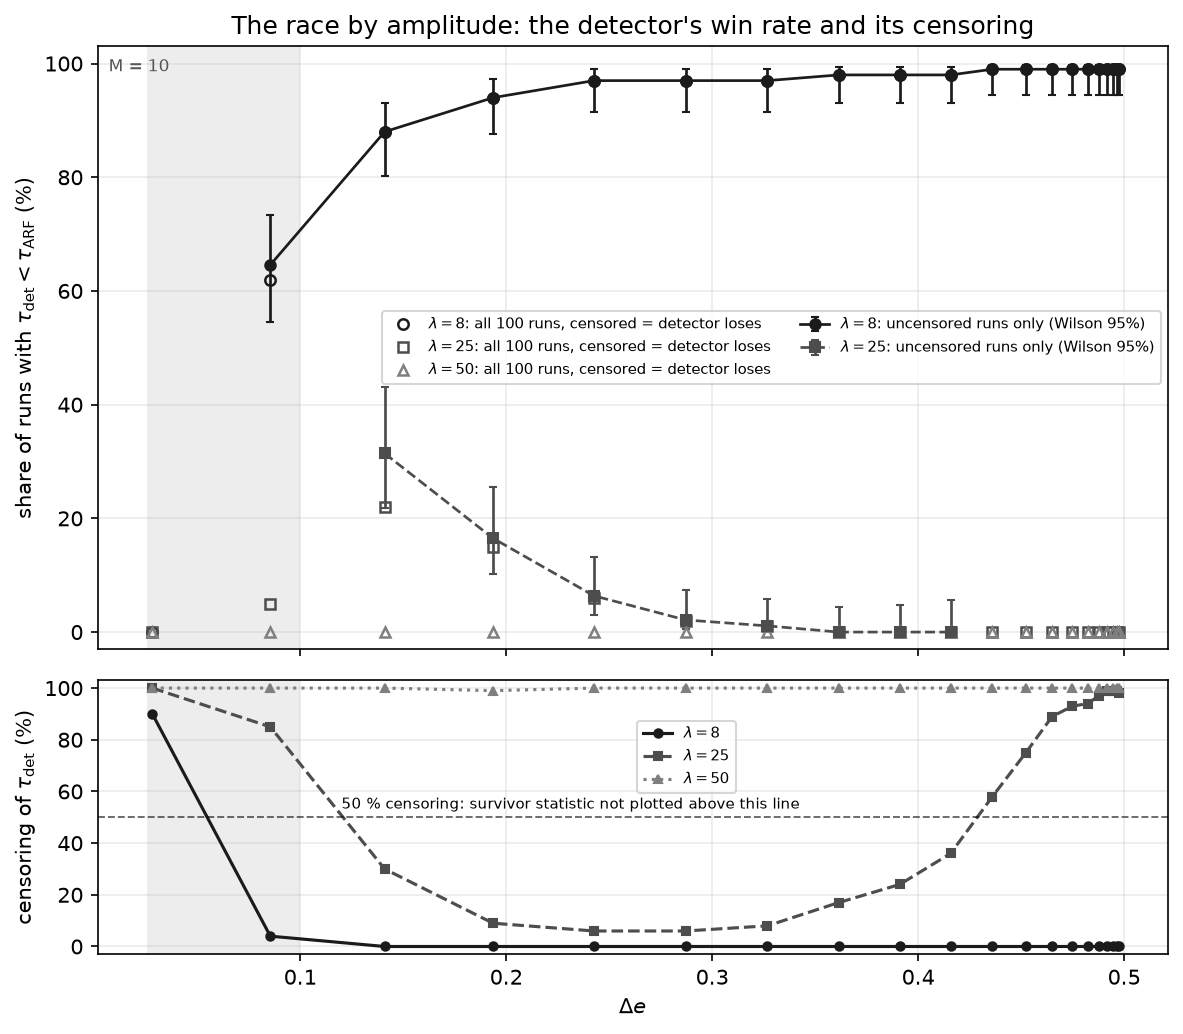
\includegraphics[width=0.9\textwidth]{resultats_R2/resultats/figures/Fig_QD_course_lambda_full.png}
  \caption{The race as a function of $(\lambda,\Delta e)$, the two quantities
  $P_{\mathrm{miss}}$ depends on. Top: share of runs in which
  $\tau_{\mathrm{det}}<\tau_{\mathrm{ARF}}$ --- the complement of $\mathrm{Miss}$ up to
  ties --- by amplitude, for $\lambda\in\{8,25,50\}$. Filled markers with error bars:
  uncensored runs only, Wilson $95\%$ interval, drawn only where the cell's censoring is
  at most $50\%$. Hollow markers: all $100$ runs, censored runs counted as detector
  losses, i.e.\ as region-2 Misses. Bottom: censoring of $\tau_{\mathrm{det}}$ in the
  same cells, with the $50\%$ line. Produced by \texttt{figures\_revision\_QCD.py}
  for Q~D.1.}
  \label{fig:course-lambda}
\end{figure}

\section{Outlook}

The Fréchet bound of Section~3 has not been evaluated on the estimated marginals
$\hat F_A$ and $\hat F_D$. Doing so would say how much is gained by knowing the
\emph{structure} of the problem rather than the marginals alone --- which is exactly the
point of Question~B: independence conditional on the stream yields a sharper law than
knowledge of the marginals alone. Given that $P_{\mathrm{miss}}$ is already point
identified here (Section~\ref{sec:measured}), this comparison is now a question about
how much the universal bound concedes, not about identifying the target.

\end{document}
